\subsection{Configuración ambiente de desarrollo y problemas enfrentados}

Este capítulo describe las diferentes etapas por las que ha atravezado el desarrollo de este sistema hasta llegar a su última iteración. Se inicia con una breve reseña de los pasos previos al desarrollo, es decir, la instalación de herramientas y configuración de la máquina de trabajo donde se desarrollaró la aplicación móvil y web. Luego, a modo de introducción, se da paso a la presentación de una aplicación básica utilizando el IDE \textit{Android Studio}, posteriormente se muestran los cuatro prototipos del sistema señidos a la metodología de desarrollo de \textit{software} elegida.\\

Las características del equipo de trabajo y dispositivo móvil para la realización y pruebas del sistema fueron:

\begin{itemize}
\item \textit{Notebook MacBook Pro}, procesador 2,5 Ghz \textit{Intel Core} i5.
\item \textit{Smartphone} Motorola Moto X, con Android 4.4.4.
\end{itemize}

Fue necesario instalar y activar algunos servicios que fueron escogidos para el proyecto. En la tabla 18 se indican las herramientas instaladas, activadas y/o servicios iniciados, junto con su versión, en la máquina de trabajo.

\begin{spacing}{1.0}
	\begin{table}[H]
		\centering
		\caption{Herramientas, estado y versión en máquina de trabajo.} 
		\begin{tabular}{|c|c|c|}
			\hline 
			\rowcolor{gray!30} &&\\
			\rowcolor{gray!30} \textbf{Herramienta} & \textbf{Acción requerida} & \textbf{Versión} \\ 
			\rowcolor{gray!30} &&\\
			\hline 
			&&\\[-0.2cm]
			Apache & Iniciar servicio & 2.4.9\\
			\hline 
			&&\\[-0.2cm]
			PHP & Activar servicio & 5.5.14 \\
			\hline 
			&&\\[-0.2cm]
			Android Studio & Descargar e instalar & 1.0 \\
			\hline 
			&&\\[-0.2cm]
			MySQL & Descargar, instalar e iniciar & 5.6.23 \\
			\hline 
			&&\\[-0.2cm]
			MySQLWorkbench & Descargar e instalar & 6.1 \\
			\hline			
		\end{tabular}
		\label{ambienteDesarrollo}
	\end{table}
\end{spacing}

Las herramientas que requerieren ser iniciadas y activadas vienen instaladas previamente en el Sistema Operativo. En cambio, las herramientas que no están incluidas fueron descargadas de su propio sitio web e instaladas posteriormente.\\ 

Durante instalación de las herramientas mencionadas no hubo mayores problemas; sin embargo, en los servicios, expuestos en la tabla anterior, se activaron e iniciaron mediante el uso de comandos a través del terminal de OS X. 

Para iniciar Apache, abrir el terminal e ingresar en modo super usuario, \textit{root}, para tener todos los permisos. En la Figura 22 se exhiben los comandos:

\begin{figure}[H]
\centering
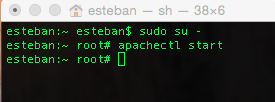
\includegraphics[scale=0.90]{images/capitulo5/apacheStart.png}
\caption{Iniciar Apache desde el terminal de OS X.}
\label{apacheStart}
\end{figure} 

Seguido de lo anterior, es recomendable corroborar que se ha iniciado Apache. Para ello, abrir el navegador web y en la barra de direcciones escribir: 'http://localhost', debe aparecer el mensaje 'It works!' como muestra la Figura 23.\\

\begin{figure}[H]
\centering
\setlength\fboxsep{0pt}
\setlength\fboxrule{0.5pt}
\fbox{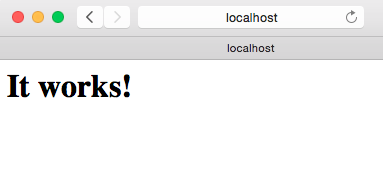
\includegraphics[scale=0.80]{images/capitulo5/localhost.png}}
\caption{Servicio Apache funcionando correctamente.}
\label{localhost}
\end{figure}

Posteriormente, se continúa con la activación de PHP. Nuevamente usando el terminal, dirigirse a la carpeta apache2: 'cd /etc/apache2/'. En esa carpeta se encuentra el archivo 'http.conf', dentro del archivo descomentar, borrar el signo '\#', la siguiente línea: 'LoadModule php5\_module libexec/apache2/libphp5.so'. Por último reiniciar Apache: 'apachectl restart'. Las figuras 24, 25 y 26 muestran lo descrito anteriormente.\\

\begin{figure}[H]
\centering
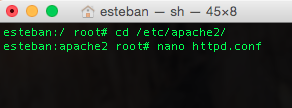
\includegraphics[scale=0.80]{images/capitulo5/httpd.png}
\caption{Acceso a carpeta apache2 y edición archivo httpd.conf.}
\label{activacionPHP}
\end{figure}

\begin{figure}[H]
\centering
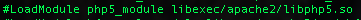
\includegraphics[scale=0.80]{images/capitulo5/libphp.png}
\caption{Habilitar PHP para Apache.}
\label{libphp}
\end{figure}

\begin{figure}[H]
\centering
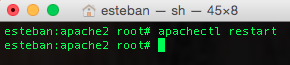
\includegraphics[scale=0.80]{images/capitulo5/apacheRestart.png}
\caption{Reiniciando Apache.}
\label{apacheRestart}
\end{figure}

Para finalizar, es importante aclarar que MySQLWorkbench\footnote{Es una herramienta visual de diseño, administración, creación y mantención de bases de datos MySQL. Más información en: \url{http://www.mysql.com/products/workbench/}}, Android Studio\footnote{\url{http://developer.android.com/sdk/index.html}} y MySQL\footnote{\url{http://dev.mysql.com/downloads/mysql/}} fueron descargados e instalados sin inconvenientes.\\

\subsection{Presentación de prototipos}

En esta sección, se muestra el crecimiento y nuevas funciones que ha logrado el sistema en las diferentes iteraciones. En cada caso se entrega una explicación de los aspectos que se consideran más importantes, y que forman parte de situaciones que exigieron interiorizarse para superar inidencias que surgieron en algunas de las etapas que se enseñan en los siguientes puntos.\\

\subsubsection{Prototipo 1: Aplicación básica en android Studio}

La primera aplicación se realizará a modo de ejercicio para corroborar que está funcionando correctamente \textit{Android Studio} y el \textit{smartphone}, para probar las aplicaciones hechas. Antes de realizar alguna acción es necesario tener el celular en modo depuración. Para esto hay que dirigirse a: Configurar -> Programador -> Depuración por USB. La Figura 27 muestra la opción que debe estar seleccionada.\\

\begin{figure}[H]
\centering
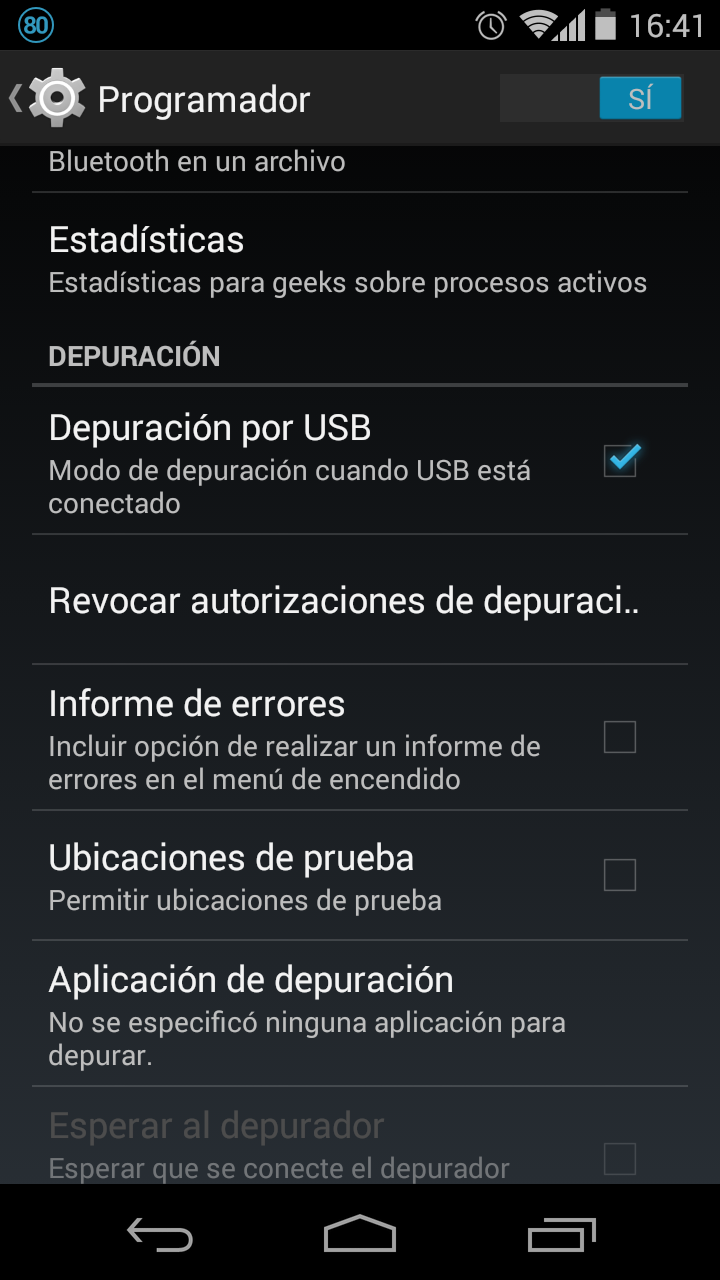
\includegraphics[scale=0.25]{images/capitulo5/modoDepuracion.png}
\caption{Modo Depuración por USB activado en \textit{Android} 4.4.4.}
\label{modoDepuracion}
\end{figure}

En la Figura 28, se puede apreciar la ventana de bienvenida de \textit{Android Studio}. Aquí es posible crear nuevos proyectos, abrir proyectos existentes, entre otras funciones.\\

\begin{figure}[H]
\centering
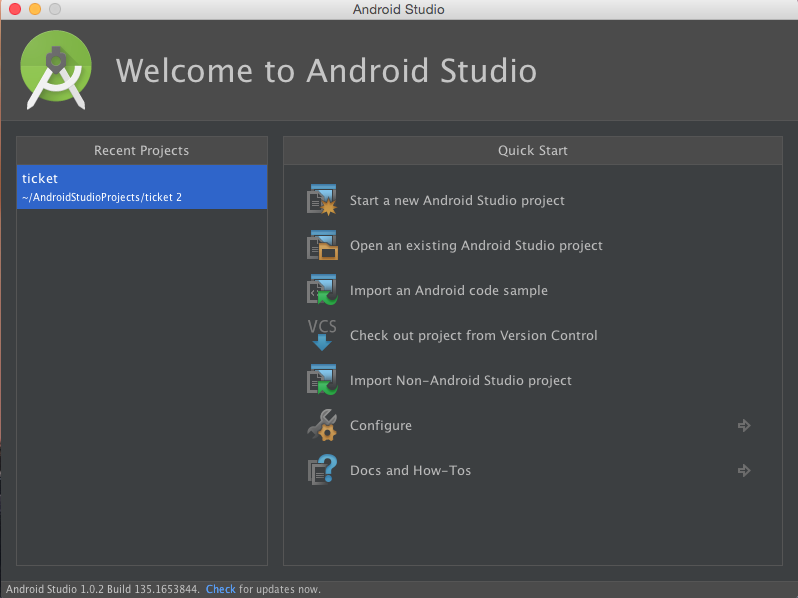
\includegraphics[scale=0.40]{images/capitulo5/androidStudio.png}
\caption{Ventana bienvenida \textit{Android Studio}.}
\label{androidStudio}
\end{figure}

En el momento que se crea un nuevo proyecto, luego de ingresar el nombre que éste tendrá, el asistente solicita elegir la versión mínima sobre la cual correrá nuestra aplicación móvil. Por lo tanto, es importante elegir correctamente, para evitar futuras complicaciones de compatibilidad cuando se cargue la aplicación en equipos que, posiblemente, tengan una versión menor a la elegida. En el menú desplegable de la Figura 29 se debe elegir una versión de API que será la versión mínima que necesitará la aplicación para ejecutarse en un \textit{smartphone}. La versión más antigua disponible en el menú es \textit{Android} 4.0.3 - \textit{IceCreamSandwich} y la más nueva es la versión reciente \textit{Android} 5.0 - \textit{Lollipop}.\\

\begin{figure}[H]
\centering
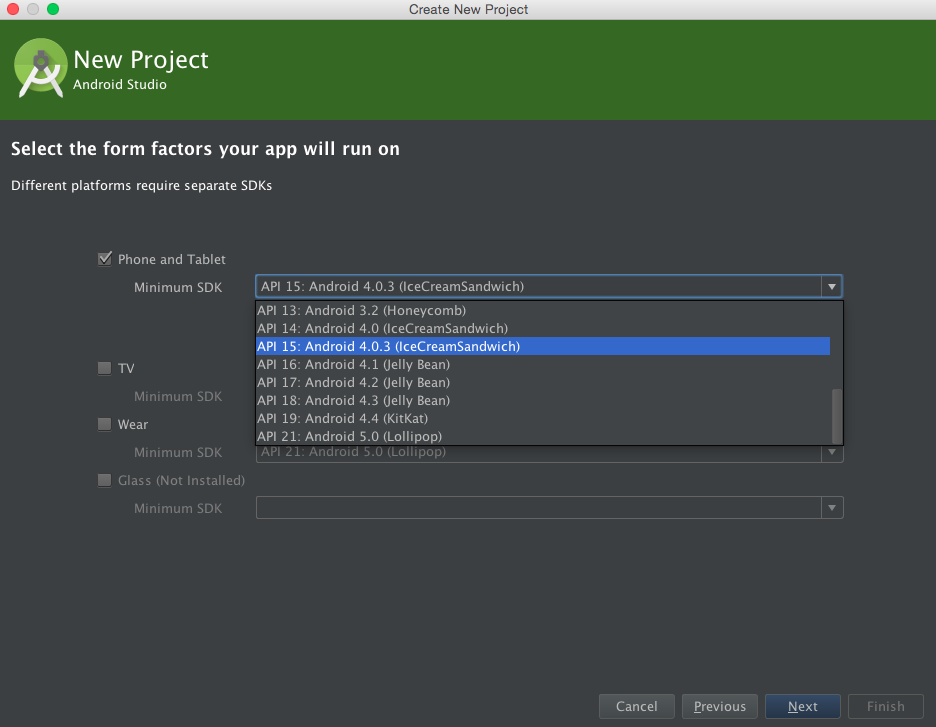
\includegraphics[scale=0.40]{images/capitulo5/minSDK.png}
\caption{Elección de API mínima requerida.}
\label{minSDK}
\end{figure}

El proyecto en el entorno de desarrollo, Figura 30, a la izquierda cuenta con un árbol para navegar y acceder a las diversas carpetas y archivos que contiene la aplicación. El código fuente de nuestro programa \textit{Android}, \textbf{controlador}, se encuentra dentro de la carpeta: app -> src -> main -> java. Es ahí donde se encuentran las clases del proyecto que dan vida a la interfaz gráfica de la aplicación, que en el patrón MVC corresponde a la \textbf{vista}. Ésta última, dentro del proyecto la ubicamos en la ruta: app -> src -> main -> res -> layout. Acá están almacenadas todas las pantallas que tendrá nuestra aplicación. A la derecha de la venta en la Figura 30 se aprecia el código fuente de la aplicación básica realizada con fines de prueba.\\

\begin{figure}[H]
\centering
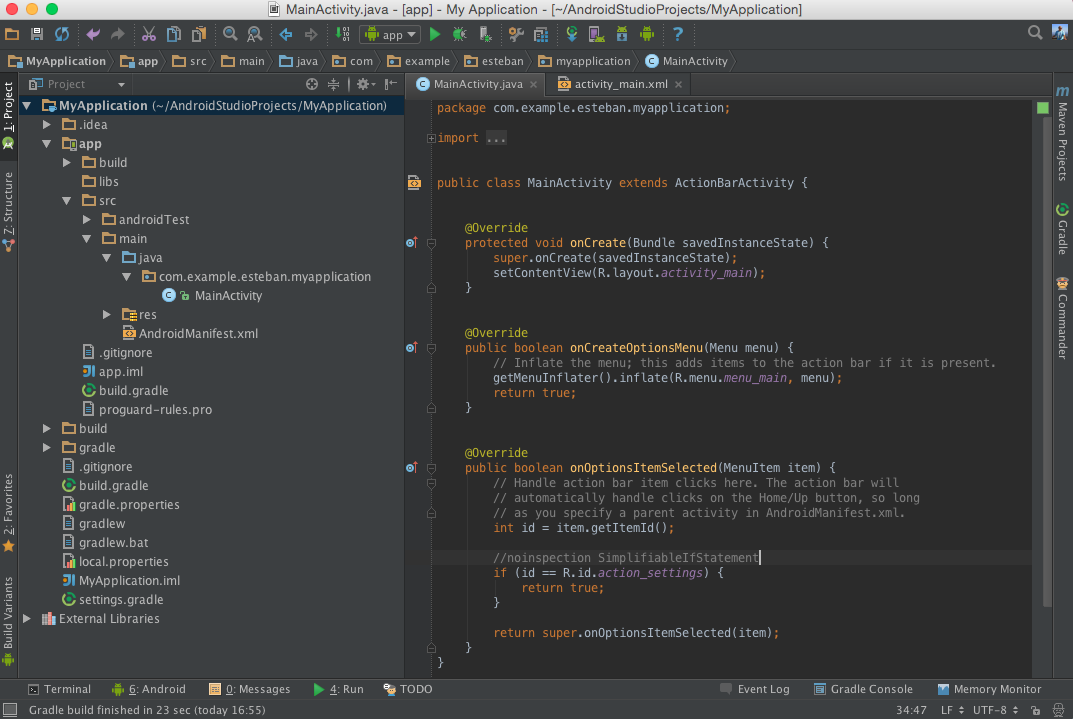
\includegraphics[scale=0.40]{images/capitulo5/proyectoAndroid.png}
\caption{Proyecto nuevo en \textit{Android Studio}.}
\label{proyectoAndroid}
\end{figure}

Luego de proceder a compilar el proyecto, y previamente haber conectado el celular al computador de trabajo, la aplicación móvil es enviada al smartphone a través del cable USB. Ya en el dispositivo ésta es instalada y ejecutada automáticamente. En la Figura 31 se ve el resultado del proyecto creado anteriormente. Debido a que no hubo inconvenientes en esta pequeña prueba, se concluye que el entorno de trabajo está listo para iniciar el desarrollo de la aplicación móvil, que forma parte del sistema propuesto como solución a la problemática antes definida en la sección 3.1 del documento.\\

\begin{figure}[H]
\centering
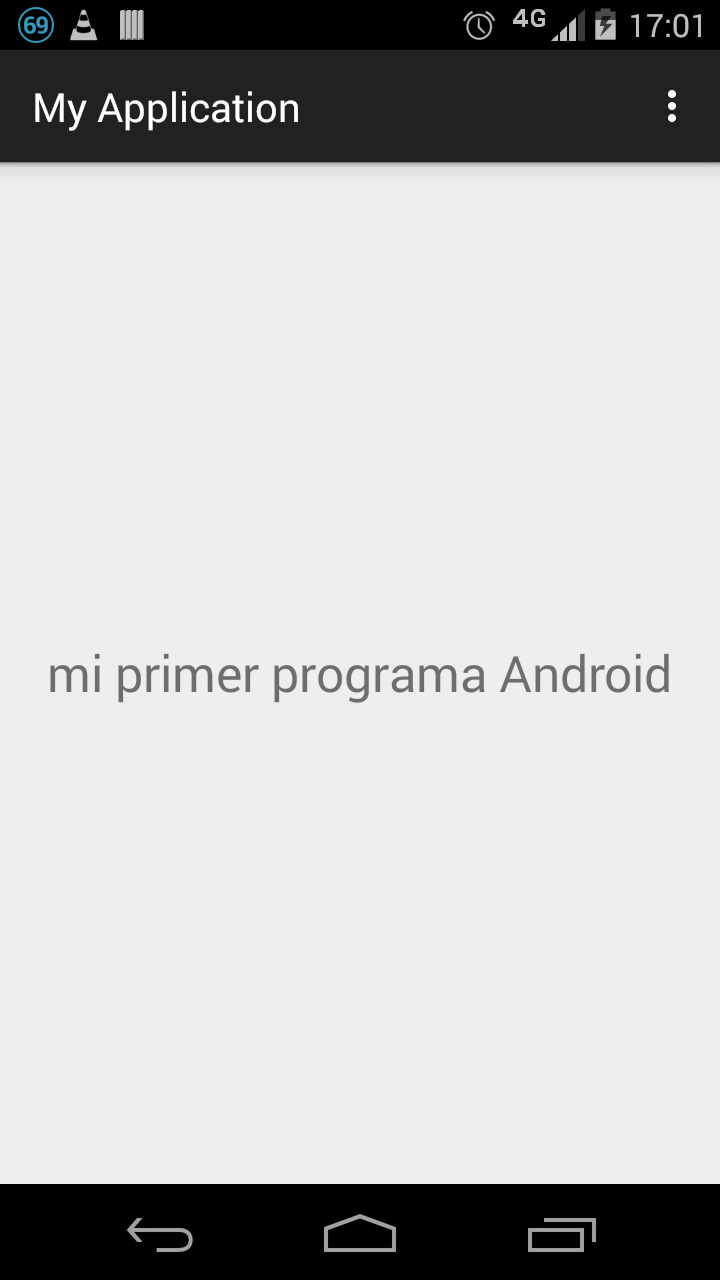
\includegraphics[scale=0.25]{images/capitulo5/primeraAplicacion.png}
\caption{Primera aplicación móvil de prueba.}
\label{minSDK}
\end{figure}

\subsubsection{Prototipo 2: Cliente y Servidor GCM}

En esta sección, se mostrará la implementación del servidor y cliente que envía y recibe mensajes, respectivamente, a través de \textit{Google Cloud Messaging}.\\  

\myparagraph{Cliente}

Antes de crear un proyecto en \textit{Android Studio} es necesario crear un proyecto, ver Figura 32, en \textit{Google Developers Console.\footnote{Es un espacio que tienen los desarrolladores de \textit{Google} para la gestión y visualización de las API de la compañía que sus proyectos utilizan. Más información en: \url{https://developers.google.com/console/help/new/}}}\\


\begin{figure}[H]
\centering
\setlength\fboxsep{0pt}
\setlength\fboxrule{0.5pt}
\fbox{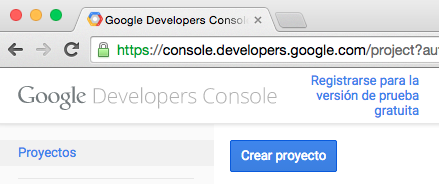
\includegraphics[scale=0.60]{images/capitulo5/gdc.png}}
\caption{Crear nuevo proyecto en Google Developers Console.}
\label{gdc}
\end{figure}

Luego de ser creado el proyecto, se desplega un resumen con información del proyecto (Figura 33), en la que aparece el \textit{PROJECT NUMBER} que corresponde a un identificador único de los proyectos creados en esta plataforma. Mas adelante será incluido en la aplicación móvil.\\

\begin{figure}[H]
\centering
\setlength\fboxsep{0pt}
\setlength\fboxrule{0.5pt}
\fbox{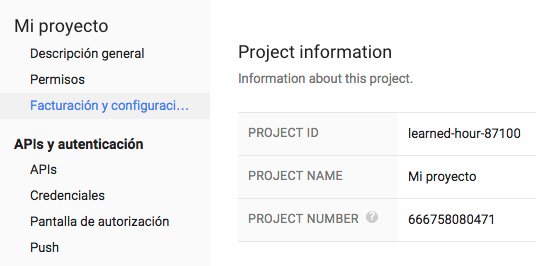
\includegraphics[scale=0.50]{images/capitulo5/resumenProyecto.png}}
\caption{Resumen proyecto.}
\label{resumenProyecto}
\end{figure}

Posteriormente es necesario habilitar APIs que provee \textit{Google} para los diferentes servicios que ofrece (\textit{Calendar, Contacts, Gmail, Google Maps Android, Google Play Game Services}, entre muchos servicios más.). Para efectos del proyecto sólo se habilitará la API \textit{Google Cloud Messaging for Android} que se puede apreciar en la Figura 34.\\

\begin{figure}[H]
\centering
\setlength\fboxsep{0pt}
\setlength\fboxrule{0.5pt}
\fbox{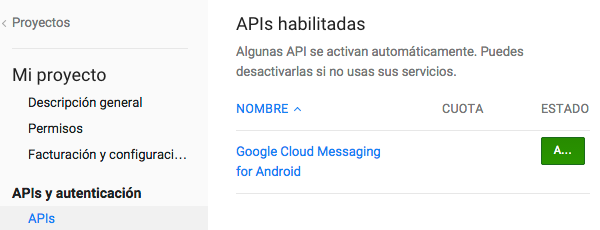
\includegraphics[scale=0.50]{images/capitulo5/API.png}}
\caption{Activación de API para proyecto.}
\label{API}
\end{figure}

Dentro de la API seleccionada, es importante crear una clave nueva para un servidor a través del cual circulan las notificaciones que sean enviadas desde el servidor del sistema. Ver Figuras 35, 36 y 37. En la Figura 38 se muestra un resumen con información a cerca del servidor creado. En la primera línea del resumen se encuentra la Clave DE LA API, que corresponde a un identificador único de dicho servidor. Este identificador al igual que el \textit{PROJECT NUMBER} serán incluidos en el sistema. \\

\begin{figure}[H]
\centering
\setlength\fboxsep{0pt}
\setlength\fboxrule{0.5pt}
\fbox{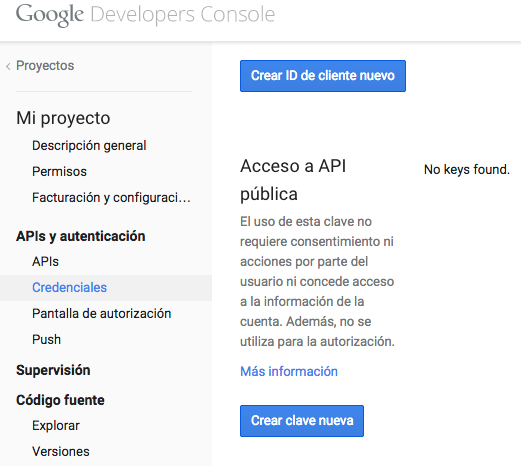
\includegraphics[scale=0.40]{images/capitulo5/claveNueva.png}}
\caption{Crear clave nueva.}
\label{cuentaNueva}
\end{figure}

\begin{figure}[H]
\centering
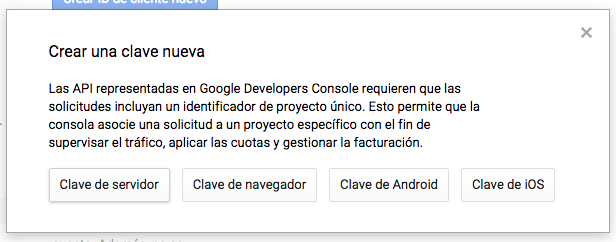
\includegraphics[scale=0.40]{images/capitulo5/cuentaNueva.png}
\caption{Crear clave nueva clave de servidor.}
\label{crearClaveNueva}
\end{figure}

\begin{figure}[H]
\centering
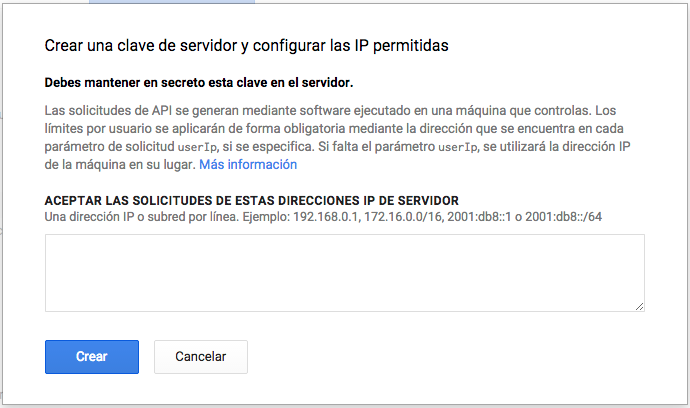
\includegraphics[scale=0.50]{images/capitulo5/crearClave.png}
\caption{Crear clave de servidor.}
\label{botonClaveNueva}
\end{figure}

\begin{figure}[H]
\centering
\setlength\fboxsep{0pt}
\setlength\fboxrule{0.5pt}
\fbox{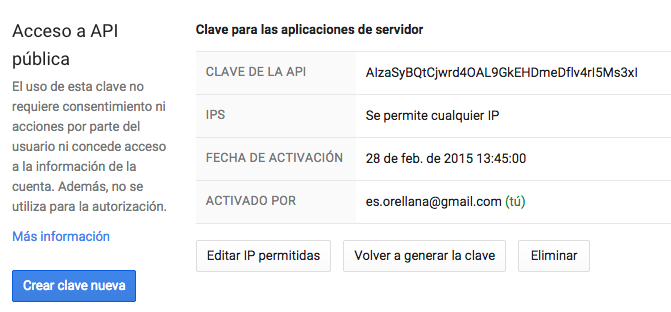
\includegraphics[scale=0.50]{images/capitulo5/resumenServidor.png}}
\caption{Resumen servidor.}
\label{resumenServidor}
\end{figure}

Dentro de \textit{Android Studio} en el \textit{SDK Manager} hay que instalar el \textit{package} de \textit{Google Play Services}, Figura 39, que contiene la libreria GCM.jar que debe ser agregada al proyecto  para que funcione la comunicación entre la aplicación \textit{Android} y los servidores de \textit{Google} desde donde vienen las notificaciones enviadas desde el servidor local.\\

\begin{figure}[H]
\centering
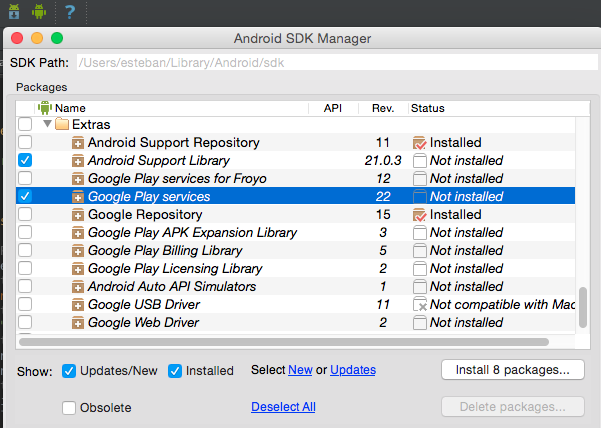
\includegraphics[scale=0.50]{images/capitulo5/sdkManager.png}
\caption{Instalación \textit{Google Play Services}.}
\label{sdkManager}
\end{figure}

En el proyecto de la aplicación cliente para \textit{Android} se tienen tres clases escritas en lenguaje java: GCMMainActivity, GCMIntentService y GCMMessageView. Entre todas se encargan de hacer posible: el registro del dispositivo. Es decir, solicitar un identificador único para el dispositivo móvil a los servidores de GCM y de esta forma poder recibir y visualizar las notificaciones. Lo anterior se muestra en la Figura 40.\\

\begin{figure}[H]
\centering
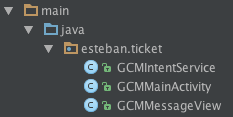
\includegraphics[scale=0.70]{images/capitulo5/proyecto.png}
\caption{Clases del proyecto.}
\label{clasesProyecto}
\end{figure}

Como se mencionó anteriormente, el \textit{PROJECT ID} sería incluido en el proyecto de \textit{Android Studio}, Figura 41. De no ser agregado este ID, la aplicación móvil queda incomunicada y sería imposible que reciba los mensajes, ya que 'no sabe' de qué proyecto debe 'escuchar' los mensajes.\\

\begin{figure}[H]
\centering
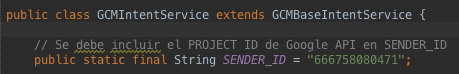
\includegraphics[scale=0.70]{images/capitulo5/idProyecto.png}
\caption{Incluir el \textit{PROJECT ID} en la aplicación.}
\label{idProyecto}
\end{figure}

La pantalla que se muestra en la Figura 42 corresponde a la aplicación creada, el botón 'Registrar Dispositivo' al ser presionado realiza la acción de solicitar el identificador asociado al dispositivo. Éste nuevo ID, sirve para asociar el celular al servidor de la API creados anteriormente. \\

\begin{figure}[H]
\centering
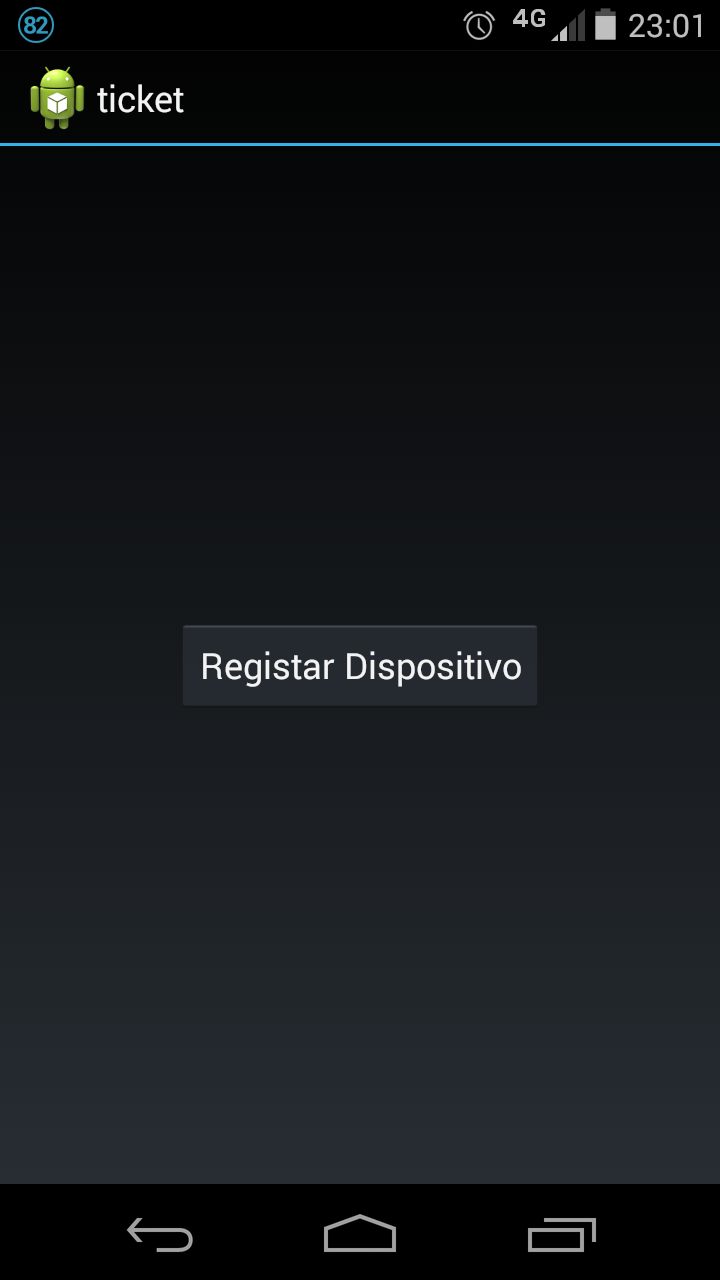
\includegraphics[scale=0.20]{images/capitulo5/registrarDispositivo.png}
\caption{Registrar dispositivo desde la aplicación.}
\label{registrarDispositivo}
\end{figure}

\myparagraph{Servidor}

El servidor está implementado en html y es la aplicación web que se mostró en las secciones anteriores. Su función es capturar datos en un formulario que posteriormente será enviado a una clase externa escrita en lenguaje PHP, la que se encarga de recibir los datos, encapsularlos y enviarlos al servidor de \textit{Google Cloud Messaging} que se creó anteriormente. En la Figuras siguientes: 43, 44 y 45 se muestra el código del mismo y después se expone el servidor en el navegador web.\\

\begin{figure}[H]
\centering
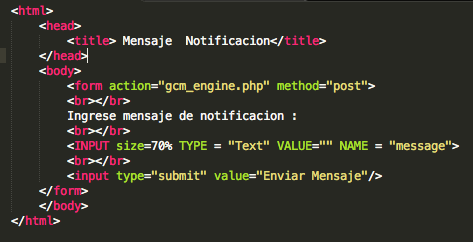
\includegraphics[scale=0.50]{images/capitulo5/codigoServidor.png}
\caption{Codigo html del Servidor.}
\label{codigoServidor}
\end{figure}

\begin{figure}[H]
\centering
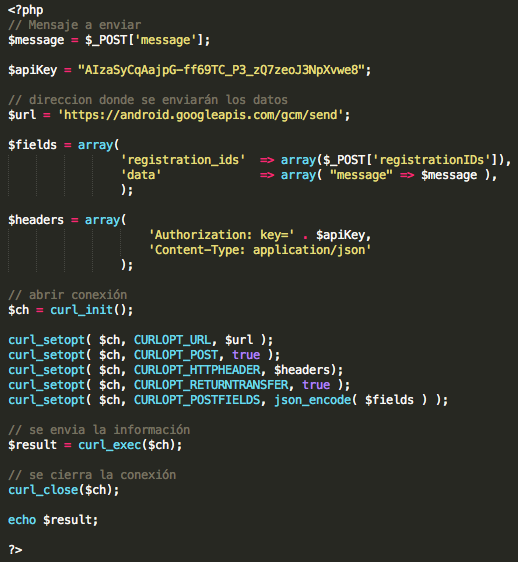
\includegraphics[scale=0.50]{images/capitulo5/codigoGCM.png}
\caption{Codigo clase gcm\_engine.php.}
\label{codigoPHP}
\end{figure}

\begin{figure}[H]
\centering
\setlength\fboxsep{0pt}
\setlength\fboxrule{0.5pt}
\fbox{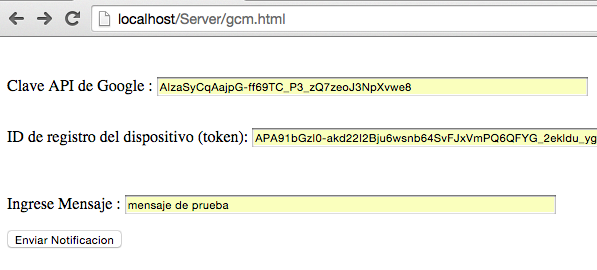
\includegraphics[scale=0.50]{images/capitulo5/servidor.png}}
\caption{Servidor.}
\label{servidor}
\end{figure}

En la Figura 45, el servidor tiene tres campos de texto. El primero, corresponde a la clave API del servidor de \textit{Google} antes creado y expuesto en la Figura 38. El segundo campo de texto, solicita que se ingrese el ID de registro del dispositivo. Éste es entregado, luego de presionar el botón 'Registrar Dispositivo' en la aplicación, ver Figura 42, por el servidor de la API creado en los pasos anteriores. En el tercer campo de texto, se debe ingresar el mensaje o notificación a enviar al o los dispositivos que tienen instalada la aplicación y se han registrado al presionar el botón antes mencionado. Por último, se debe presionar el boton 'Enviar Notificación' y el mensaje será enviado inmediatamente y podrá ser visualizado en el dispositivo móvil. Ver Figuras 46 y 47.\\

\begin{figure}[H]
\centering
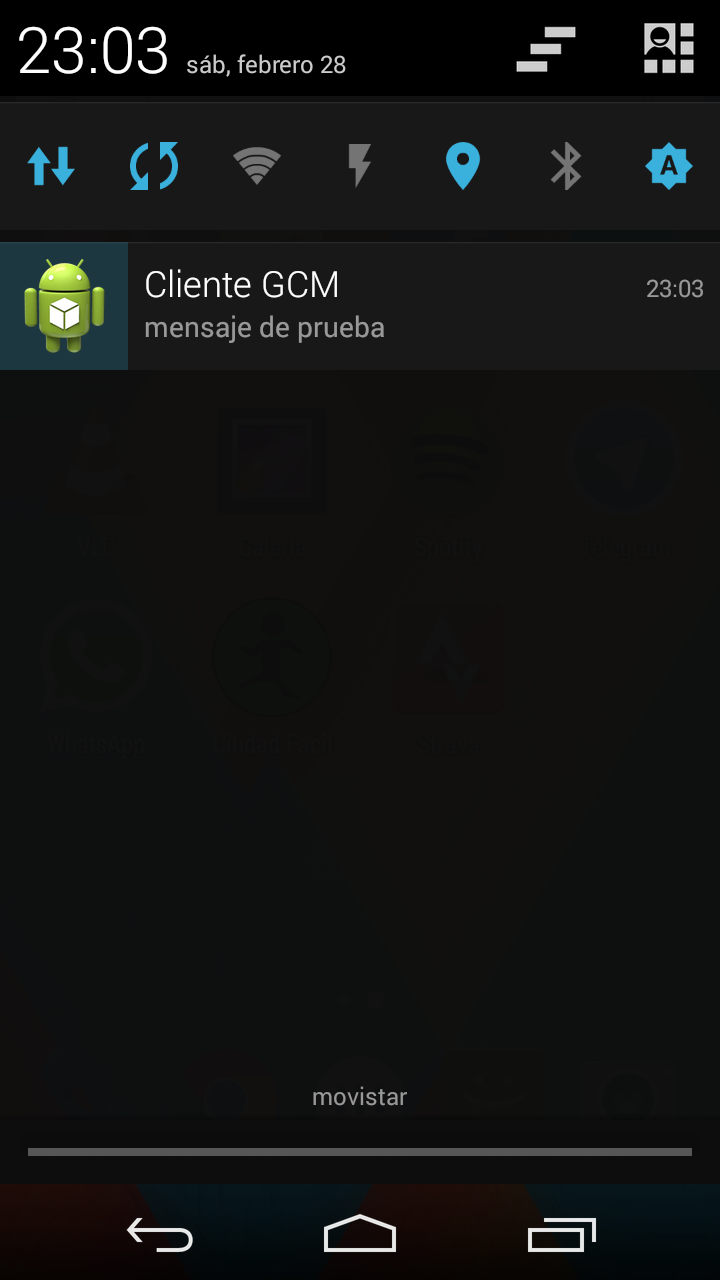
\includegraphics[scale=0.20]{images/capitulo5/notificacion.png}
\caption{Notificación \textit{Push} recibida.}
\label{notificacion}
\end{figure}

\begin{figure}[H]
\centering
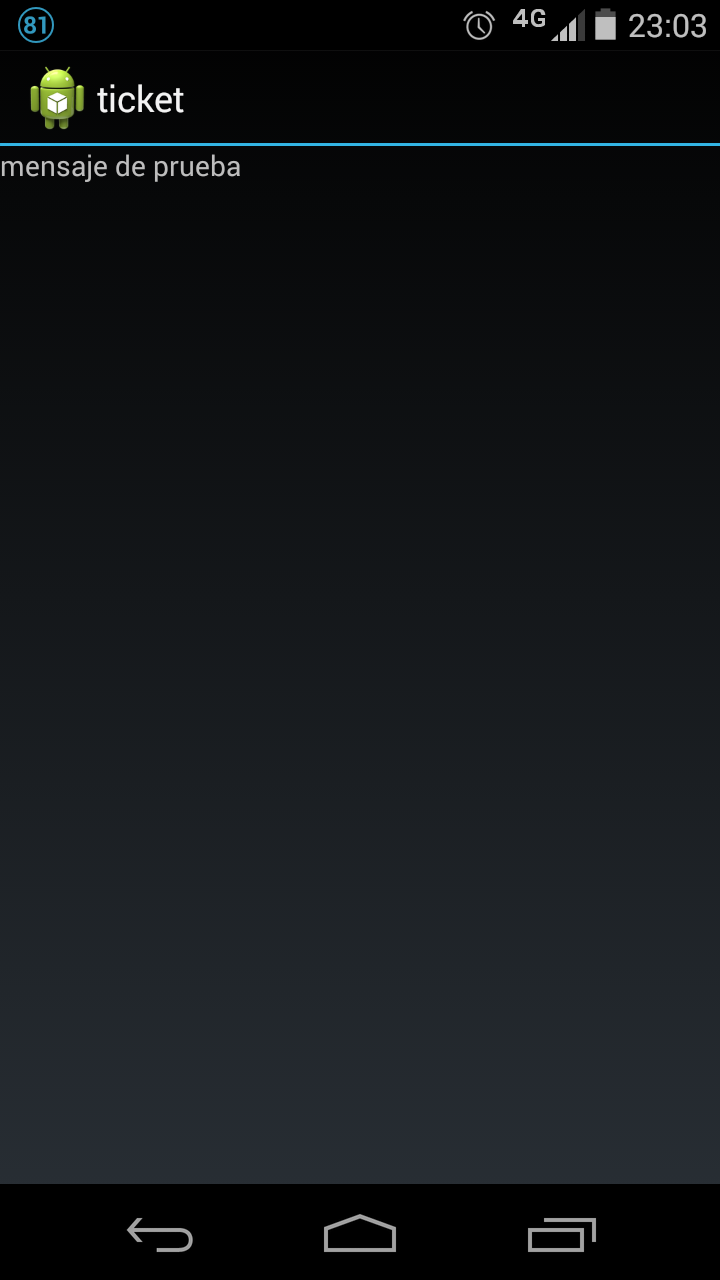
\includegraphics[scale=0.20]{images/capitulo5/notificacionApp.png}
\caption{Visualizacion contenido de notificación.}
\label{notificacionContenido}
\end{figure}

En este ítem se ha explicado paso por paso como se implementó este primer prototipo. Además, se resuelve una parte escencial de todo el sistema propuesto como solución a la problemática definida.\\

\subsubsection{Prototipo 3: Comunicar Android y MySQL}

Una forma de comunicar una aplicación \textit{Android} con una base de datos externa, que se encuentre en una máquina remota, es utilizando servicios web y un formato de intercambio de datos como es JSON\footnote{Estos conceptos y características fueron tratados con anterioridad en las secciones 2.1.4 y 3.4.2}. En la sección 2.1.4 - \textit{Web Service}, se explicó como el es flujo de datos entre: una aplicación \textit{Android} - PHP - MySQL.\\

Por el lado de la aplicación \textit{Android}, se agregaron funciones y clases al proyecto que realizan la tarea de capturar datos y enviarlos al servicio web 'index.php' ubicado en la estación de trabajo que a su vez juega el papel de servidor externo. En la Figura 48 se aprecia la misma pantalla de la aplicación pero, ahora el boton envía datos al servidor para que sean almacenados. Los datos que el celular envía a MySQL son: IMEI, clave API de \textit{Google} \textit{(token)}, lo anterior aparece en las Figuras 48, 49, 50 y 51.\\

\begin{figure}[H]
\centering
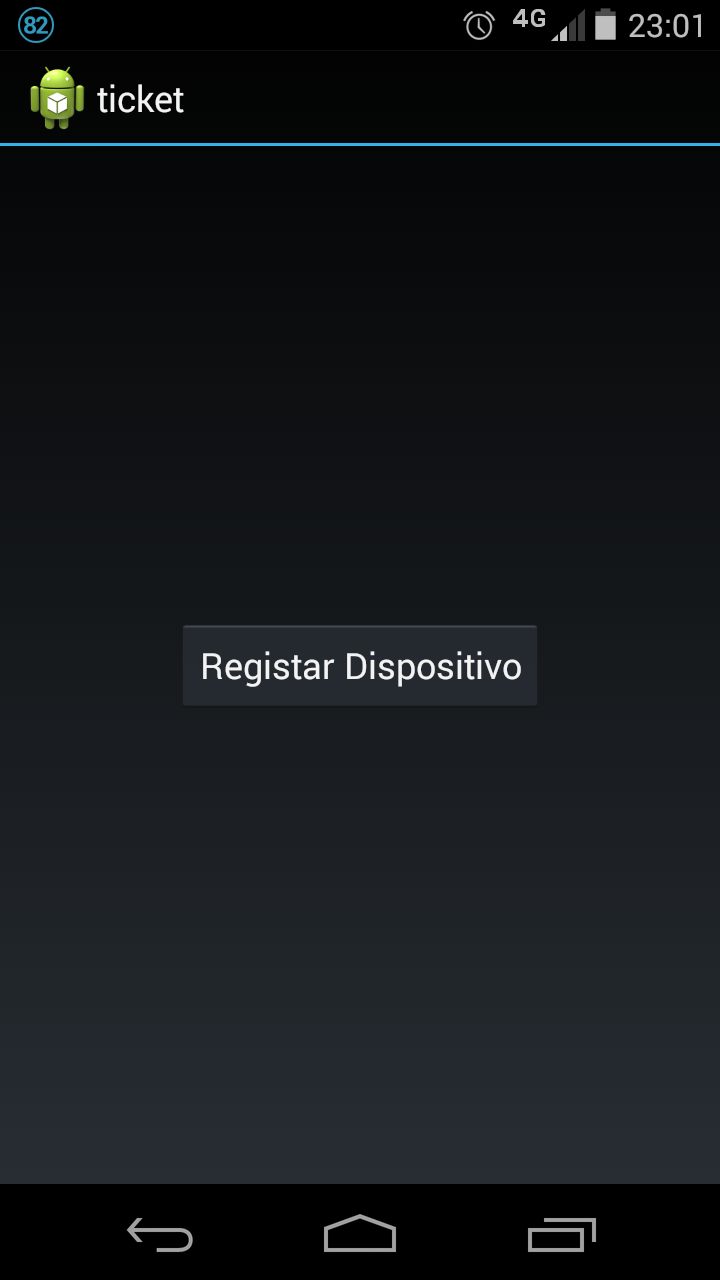
\includegraphics[scale=0.20]{images/capitulo5/registrarDispositivo.png}
\caption{Registrar dispositivo en MySQL.}
\label{registrarDispositivo}
\end{figure}

\begin{figure}[H]
\centering
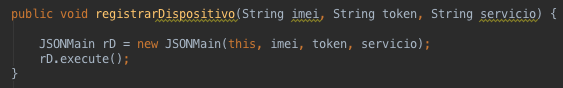
\includegraphics[scale=0.70]{images/capitulo5/funcionesAppRD.png}
\caption{Código de función registrar dispositivo.}
\label{registrarDispositivo}
\end{figure}

\begin{figure}[H]
\centering
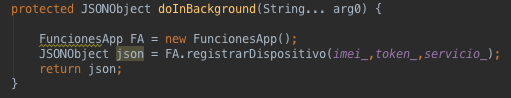
\includegraphics[scale=0.70]{images/capitulo5/JSONMain.png}
\caption{Código clase asíncrona JSONMain.}
\label{registrarDispositivo}
\end{figure}

\begin{figure}[H]
\centering
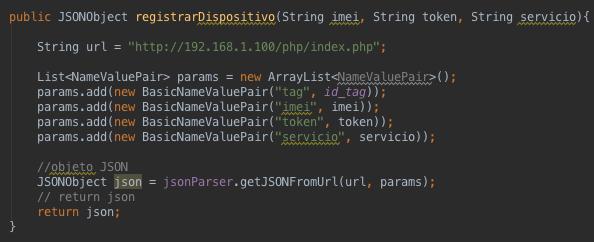
\includegraphics[scale=0.70]{images/capitulo5/funcionRD.png}
\caption{Código de función registrarDispositivo() en clase FuncionesApp().}
\label{registrarDispositivo}
\end{figure}

Los datos cuando son enviados con JSON al servidor central llegan al webservice que tiene por nombre: index.php (en la Figura 51, se aprecia la variable 'url' que contiene la ubicación de éste.) y que a través del método POST recibe entre los datos una variable llamada 'tag' que sirve para discriminar que método debe ser utilizado dentro del mismo para realizar alguna tarea específica. Ver Figura 52.\\

\begin{figure}[H]
\centering
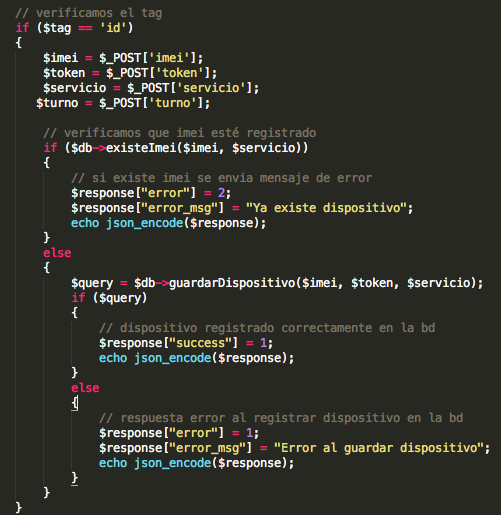
\includegraphics[scale=0.70]{images/capitulo5/index.png}
\caption{Porción de código de servicio web.}
\label{registrarDispositivo}
\end{figure}

En la Figura 52 se muestra que se realiza una instancia de la función 'guardarDispositivo()' y se le pasan como argumentos los datos enviados desde el dispositivo móvil para ser almacenados. Tal método, se encuentra en la clase PHP DB\_Functions.php. Esta clase se encarga de comunicarse directamente con la base de datos MySQL, ya sea para realizar una consulta, \textit{SELECT}, o guardar información, \textit{INSERT}. En la Figura 53 se puede ver la implementación de un \textit{INSERT} con la información recibida.\\

\begin{figure}[H]
\centering
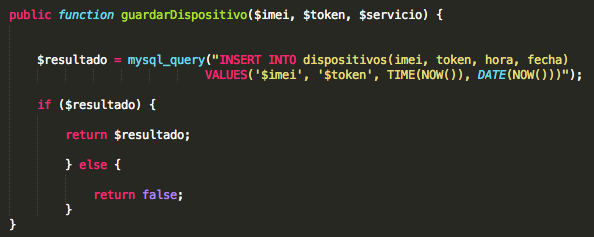
\includegraphics[scale=0.60]{images/capitulo5/guardarDisp.png}
\caption{Código de función guardarDispositivos() en clase DB\_Functions.PHP.}
\label{registrarDispositivo}
\end{figure}

Se puede ver en la Figura 54 que los datos han sido almacenados correctamente en la base de datos que se encuentra en el servidor central.\\

\begin{figure}[H]
\centering
\setlength\fboxsep{0pt}
\setlength\fboxrule{0.5pt}
\fbox{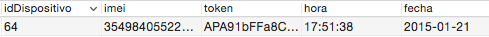
\includegraphics[scale=0.80]{images/capitulo5/MySQL.png}}
\caption{Datos almacenados correctamente en MySQL.}
\label{registrarDispositivo}
\end{figure}


\subsection{Solución final}

la solución final es el resultado de la cuarta y última iteración del proyecto, de acuerdo al ciclo de vida elegido. Así como fueron descritos anteriormente los prototipos, a continuación en este apartado se describirán las diferentes partes que forman el sistema y sus características.

\subsubsection{Servidor central}

El servidor central contiene los servicios que actuan como orquestadores del sistema definitivo. Aquí se encuentra la base de datos MySQL, el servicio web (index.php) y la aplicación web (GCM.php).\\ 

\subsubsection{Monitor}

El monitor del sistema tiene por objetivo mostrar los dos últimos números que están siendo atendidos en servicios distintos. Esta pantalla estará ubicada en un televisor ubicado en una zona visible para que los clientes puedan visualizar la información. Se actualiza cuando un número es llamado al módulo de atención. La Figura 55 muestra lo mencionado.

\begin{figure}[H]
\centering
\setlength\fboxsep{0pt}
\setlength\fboxrule{0.5pt}
\fbox{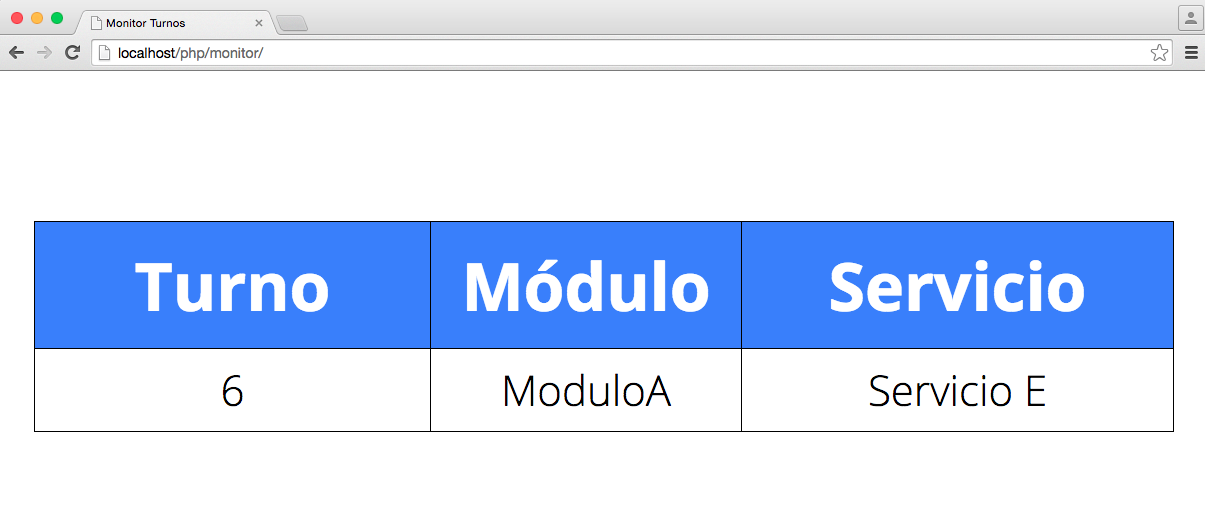
\includegraphics[scale=0.35]{images/capitulo5/monitor.png}}
\caption{Monitor del sistema.}
\label{registrarDispositivo}
\end{figure}

\subsubsection{Aplicación Web}

En la aplicación web es posible seleccionar mediante los menú desplegables el servicio y módulo de atención, ver Figura 56. Lo anterior, sirve para filtrar los mensajes que serán enviados, éstos sólo llegarán a los celulares que tienen un turno de atención en el servicio que permanece seleccionado. Por ejemplo, si está seleccionado el 'Servicio A' y se hace click en el botón 'Siguiente Turno', llegará una notificación a todos los dispositivos que hayan sacado un turno para ese servicio. En la misma figura, abajo es posible mirar el turno actual que está siendo atendido. Existe una barra de menú con diferentes opciones. En 'Reportes' es posible generar reportes con estadísticas relacionadas con el flujo de atención en los diferentes servicios. En 'Monitor' se da la posibilidad que se conozca lo mismo que están viendo los clientes. En la opción 'Configurar', están las opciones para agregar nuevos servicios y módulos de atención.

\begin{figure}[H]
\centering
\setlength\fboxsep{0pt}
\setlength\fboxrule{0.5pt}
\fbox{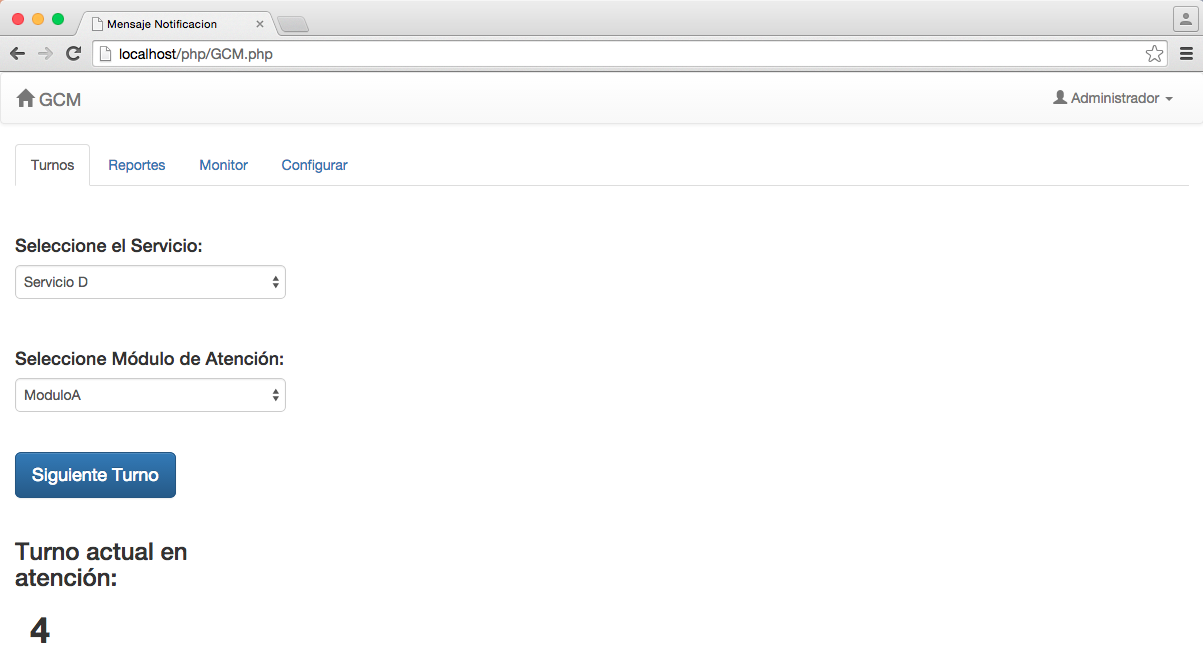
\includegraphics[scale=0.35]{images/capitulo5/gcm.png}}
%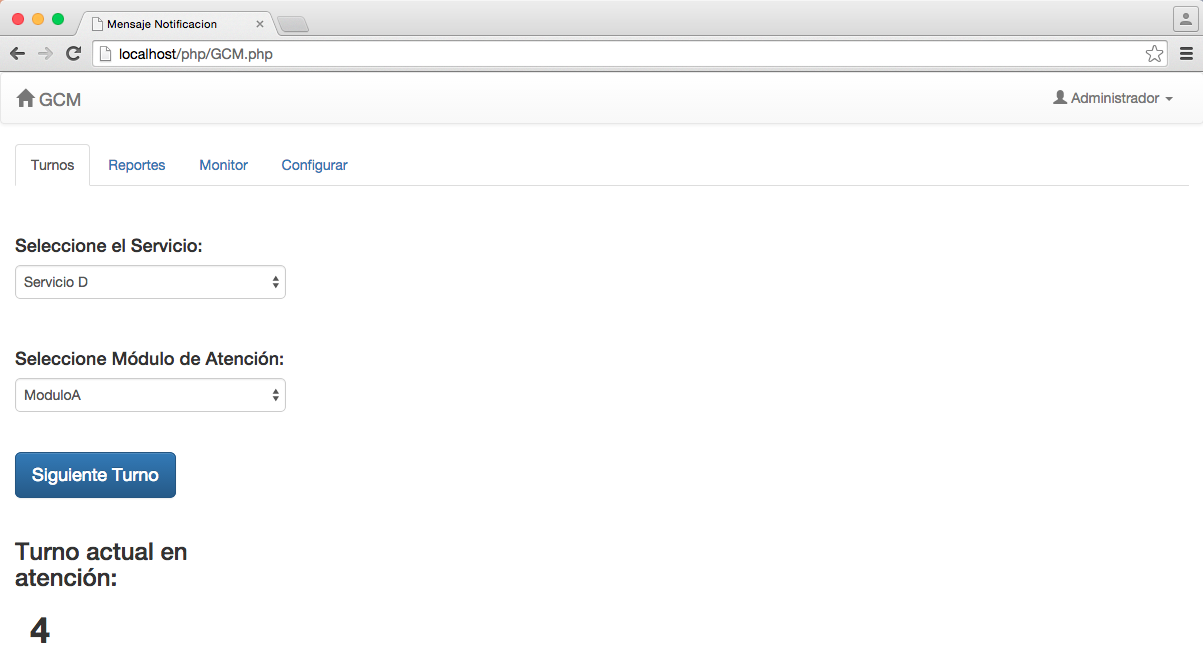
\includegraphics[scale=0.35]{images/capitulo5/gcm.png}
\caption{Aplicación web.}
\label{registrarDispositivo}
\end{figure}

\subsubsection{Aplicación Móvil}

En las siguientes Figuras: 57, 58, 59 y 60, se presentan las pantallas que tiene la aplicación móvil. Sus funciones fueron explicadas anteriormente en el Caso de Uso Real CU03 en la sección 4.5.1.\\

En la Figura de abajo, a la izquierda se aprecia la pantalla principal de la aplicación. Se dispone de botones en donde cada uno corresponde a un tipo de servicio que proporciona el centro de atención. A la derecha, está la misma ventana pero se exhibe el menú que aparece luego de presionar los 'tres puntos verticales' en la esquina superior derecha de la pantalla. Cada opción lleva a una nueva pantalla que contiene: 


\begin{itemize}
\item \textbf{Turno:} Abre la pantalla donde se muestra el turno de atención y el servicio correspondiente donde se obtuvo un ticket.
\item \textbf{Notificaciones:} Abre una pantalla de la aplicación que muestra el último mensaje enviado desde el servidor central, contiene información del estado de avance de la fila de espera.
\item \textbf{Información:} Se abre una pantalla que entrega información sobre el proyecto.
\end{itemize}


\begin{figure}[H]
\centering
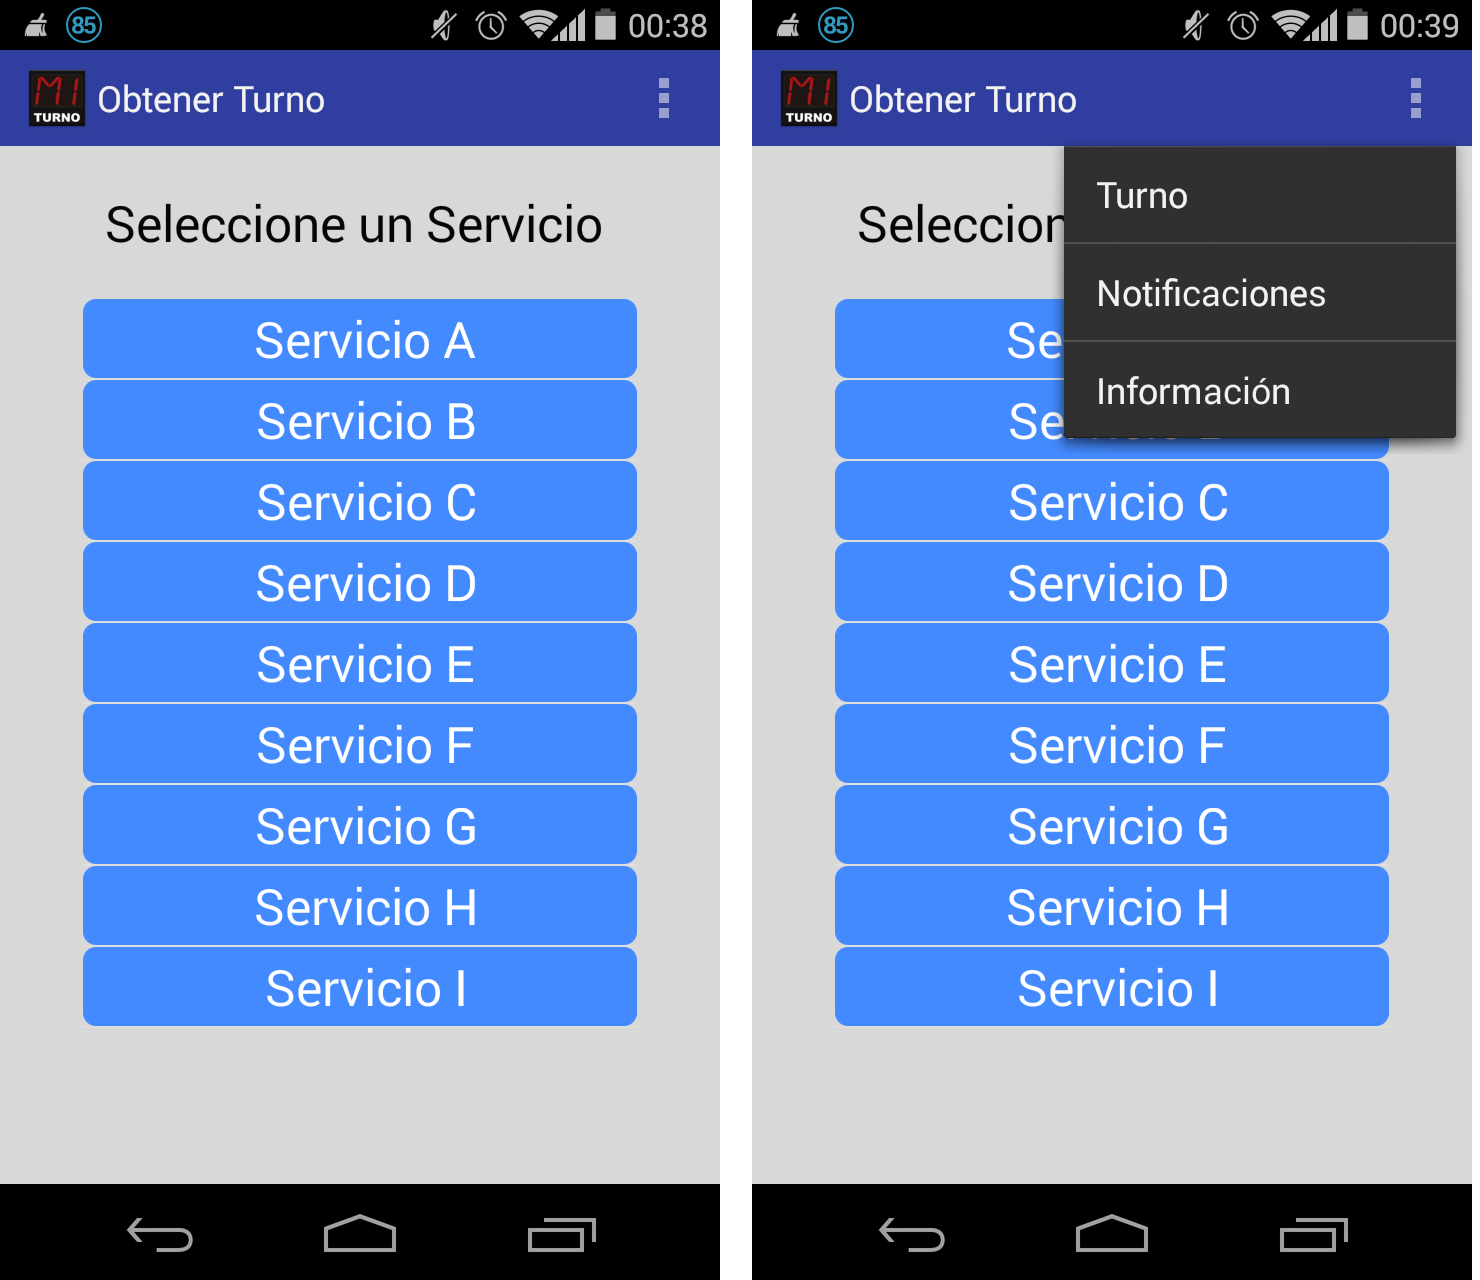
\includegraphics[scale=0.30]{images/capitulo5/obtenerTurno.png}
\caption{Pantalla principal 'Obtener Turno', a la derecha, y 'Menú' de opciones, a la izquierda,.}
\label{obtenerTurnoMenu}
\end{figure}

\begin{figure}[H]
\centering
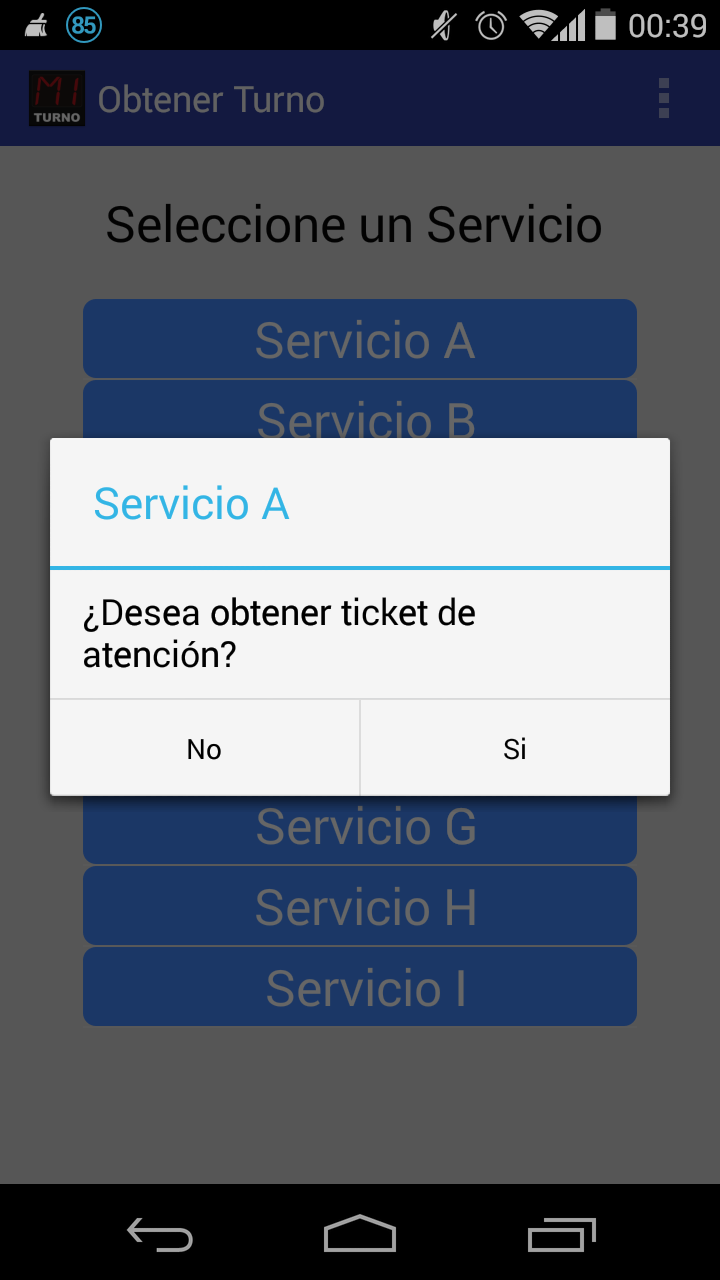
\includegraphics[scale=0.25]{images/capitulo5/dialogo.png}
\caption{Dialogo confirmación obtener turno.}
\label{dialogo}
\end{figure}

\begin{figure}[H]
\centering
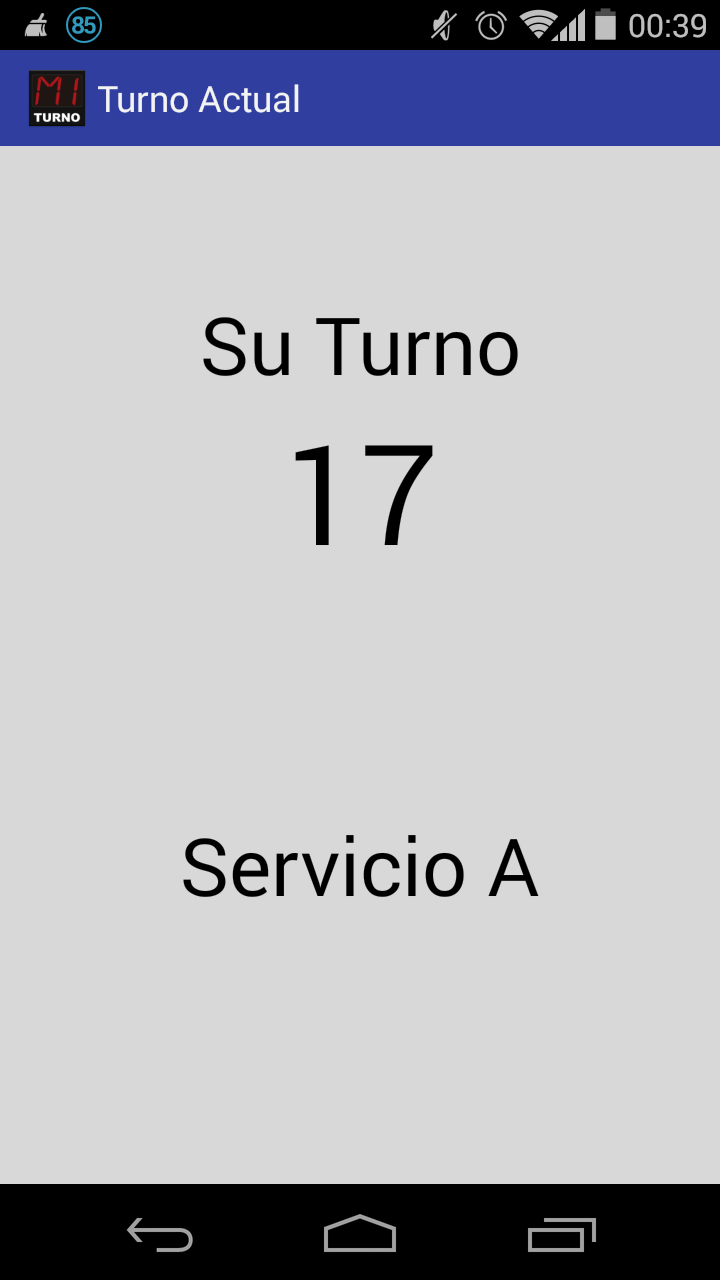
\includegraphics[scale=0.25]{images/capitulo5/turnoActual.png}
\caption{Pantalla 'Turno Actual'.}
\label{turnoActual}
\end{figure}

\begin{figure}[H]
\centering
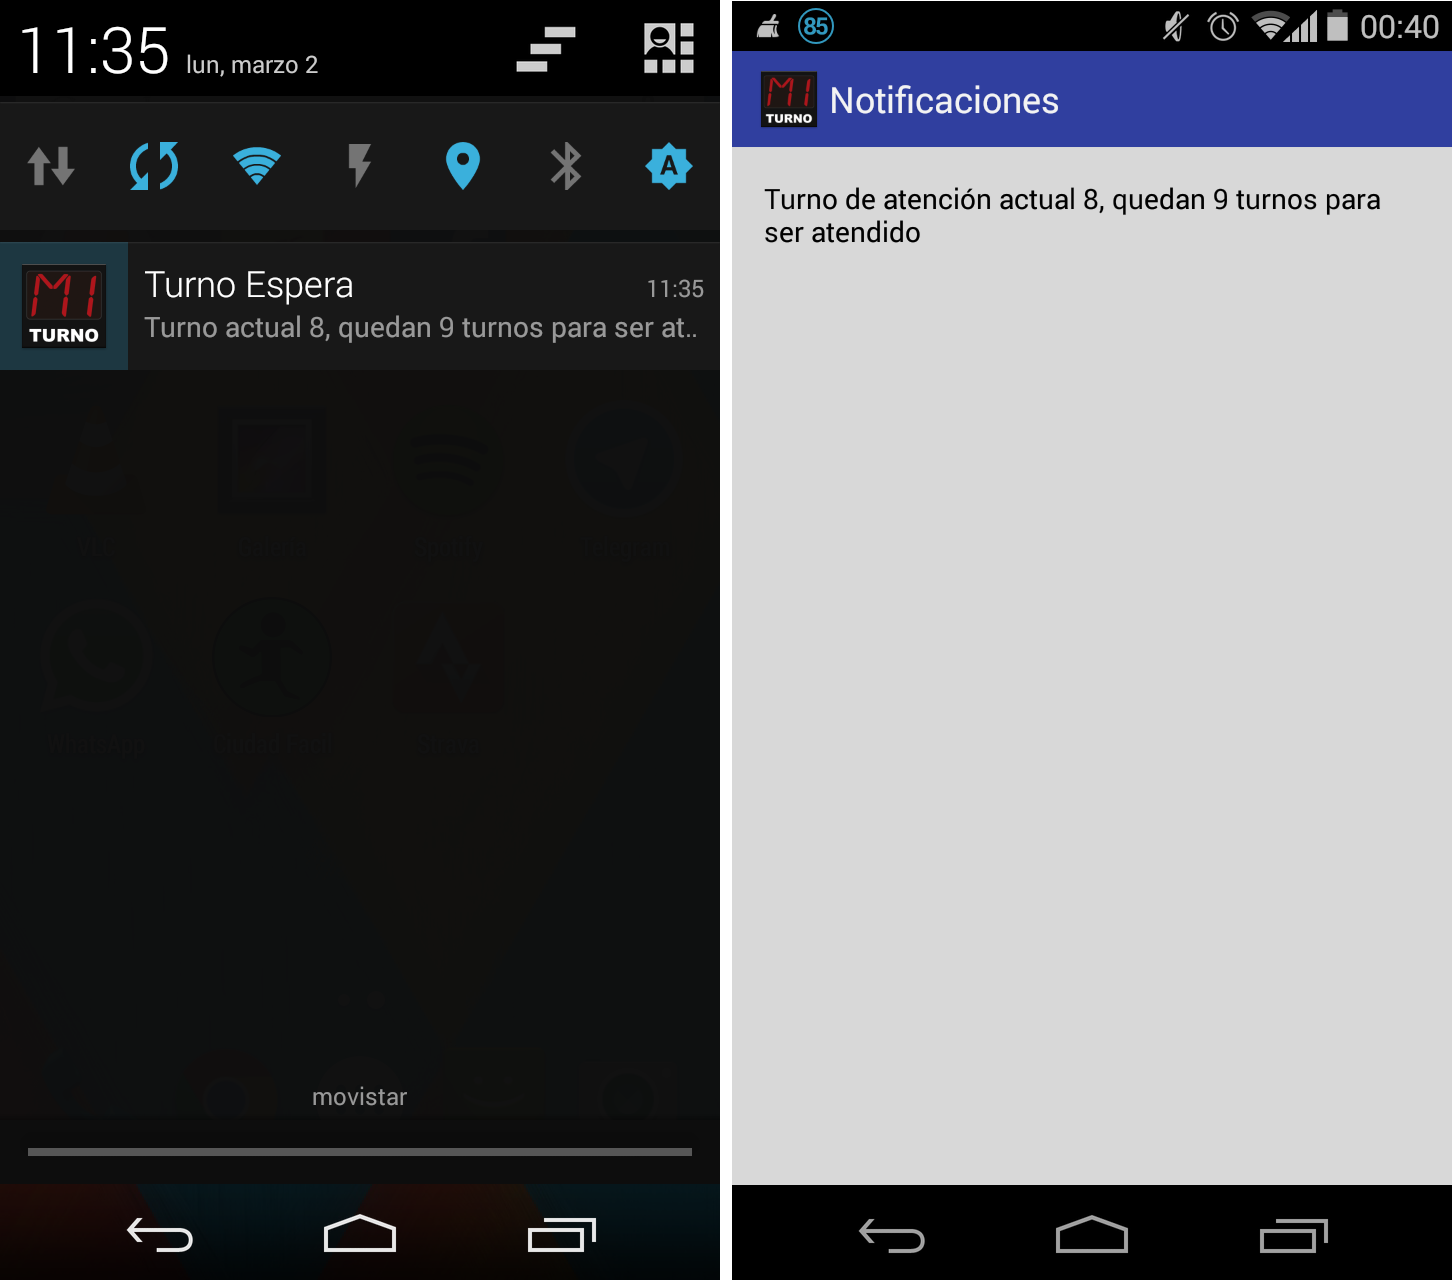
\includegraphics[scale=0.30]{images/capitulo5/notificaciones.png}
\caption{Pantalla con Notificación Push, a la izquierda. Visualización de la Notificación a la derecha.}
\label{notificaciones}
\end{figure}

%\myparagraph{Servicios de Google}


